\chapter{GEP-NEAT}\label{chapter:gep_neat}
This chapter covers GEP-NEAT, a blend between NEAT (covered in Chapter \ref{sec:ne_neat}) and gene expression programming (covered in Chapter \ref{chapter:gep}). An introduction to GEP-NEAT is given in Section \ref{sec:gep_neat_introduction}. The proposed algorithm is explained in-depth in Section \ref{sec:gep_neat_proposed_algorithm}, after which the prototype implementation is discussed in Section \ref{sec:gep_neat_protoype_implementation}. Finally, the prototype is applied to a few problems to benchmark the algorithm's performance in Section \ref{sec:gep_neat_model_validation}.

\section{Introduction}\label{sec:gep_neat_introduction}
As discussed in Chapter \ref{chapter:neuroevolution}, neuroevolution explores innovative strategies for optimising artificial neural networks (ANNs) using evolutionary algorithms (see Chapter \ref{chapter_ea}). Unlike conventional training methods such as backpropagation and gradient descent, which rely on differentiable loss functions and gradient-based updates, neuroevolution leverages Darwinian principles to evolve the topology of the neural network along with its weights and biases. This allows for the discovery of novel topologies, activation functions, and hyperparameters that may not be easily accessible through traditional approaches.

\parbreak\noindent A prominent example of this is the NEAT algorithm (Chapter \ref{sec:ne_neat}), which evolves both the structure and weights of neural weights simultaneously. NEAT's speciation mechanism preserves diversity and protects innovative structures during evolution, but one of its main challenges lies in its computational cost, largely due to the need for topological sorting during network evaluation, which makes the genotype-phenotype mapping and forward propagation computationally expensive. Nevertheless, NEAT's ability to operate without requiring differentiable functions makes it particularly well-suited for environments where gradient information is unaccessable.

\parbreak\noindent Building on these ideas, Gene Expression Programming (GEP) and its extension GEP-NN offer alternative evolutionary approaches that combine the global search capabilities of genetic algorithms with the expressive, tree-based representations of genetic programming. GEP introduces a novel genotype-to-phenotype mapping using Karva notation, enabling the evolution of complex, non-linear structures such as expression trees.

\parbreak\noindent The proposed algorithm, GEP-NEAT, integrates the representational power of GEP with the structural evolution principles of NEAT. It introduces several enhancements, including a reworked system for tracking innovation numbers, inspired by Richard Dawkins' concept of the meme. This mechanism enables more effective selection and mutation by identifying and preserving useful substructures across generations. Furthermore, GEP-NEAT addresses a key limitation in earlier GEP-based models by introducing a method for embedding bias information directly into the chromosome, thereby improving the expressiveness and learning capacity of evolved networks.

\section{Proposed Algorithm}\label{sec:gep_neat_proposed_algorithm}
\subsection{Evolutionary Life Cycle}
The goal of GEP-NEAT is to integrate the expressive representational capabilities of Karva notation from GEP with the neuroevolutionary mechanisms of NEAT, particularly its speciation and innovation tracking strategies. This hybrid approach aims to evolve neural network populations more effectively by combining the strengths of both paradigms.

\parbreak
\begin{figure}[H] % Use [H] to suppress floating and place the figure/table exactly where it is specified in the text
	\centering % Horizontally center the figure on the page
	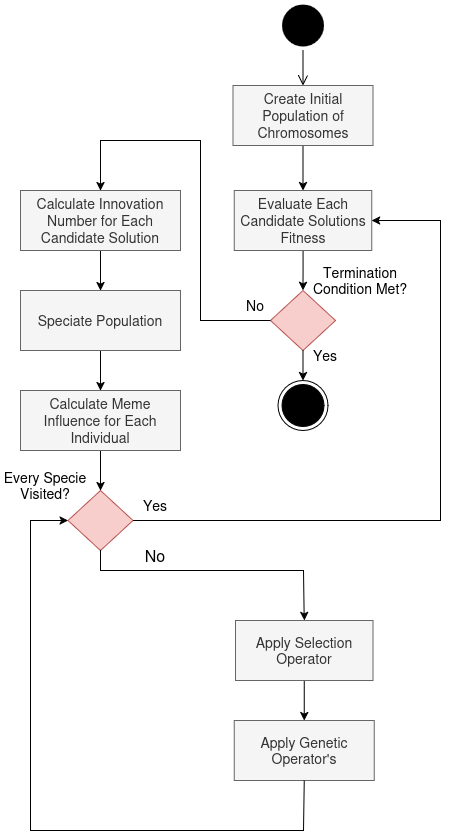
\includegraphics[width=0.65\textwidth]{Figures/chapter_gep_neat/gep_neat_framework.png} % Include the figure image
	\caption{Evolutionary Lifecycle of GEP-NEAT}
	\label{fig:gep_neat_framework} % Unique label used for referencing the figure in-text
\end{figure}

\parbreak\noindent At a high level, both NEAT and GEP follow a similar evolutionary cycle, that is, intialising a population, representing chromosomes, evaluating fitness, applying genetic operators, and iterating until a termination condition is met. The two approaches however diverge significantly in their internal mechanisms and innovations. NEAT introduces a sophisticated speciation mechanism, where historical gene information is tracked using innovation numbers. These are stored in a lookup table and used to calculate compatibility distance between individuals, allowing the population to be divided into species that evolve in parallel within their own niches (\cite{stanley2002evolving}).

\parbreak\noindent In contrast, GEP adheres more closely to the traditional genetic algorithm framework but distinguishes itself through a rich set of genetic operators that promote diversity and facilitate the emergence of reusable substructures, or building blocks, within chromosomes (\cite{ferreira2006gene}). Its use of Karva notation ensures syntactically valid expressions, making it particularly well-suited for evolving complex, non-linear representations.

\parbreak\noindent GEP-NEAT draws inspiration from both of these methodologies to form a unified framework, as illustrated in Figure \ref{fig:gep_neat_framework}. It leverages NEAT's innovation tracking and speciation to maintain diversity and protect novel structures, while adopting GEP's flexible chromosome representation to enable the evolution of expressive and structurally diverse neural networks.

\subsection{Representation}\label{sec:gep_neat_representation}
NEAT-GEP draws inspiration from the genotype-to-phenotype mapping introduced in Gene Expression Programming (GEP), particularly through the use of Karva notation, however, several modifications have been made to enhance the representation, starting with the adoption of prefix tree-style encoding. In traditional GEP, k-expressions are converted into expression trees by reading the linear string from left to right and top to bottom. While this method ensures syntactic correctness, it can become computationally expensive, especially when evaluating large populations or complex expressions since the expression tree must first be constructed from the expression string during each fitness evaluation. 

\parbreak\noindent As discussed in Chapter \ref{chapter:gep}, alternative encoding schemes such as prefix and postfix notation have been explored to address this limitation. On such approach, P-GEP, encodes linear chromosomes in prefix form. This representation improves the preservation of meaningful substructures during operations like crossover and mutation, which in turn supports more efficient and targeted exploration of the search space.

\parbreak\noindent Figure \ref{fig:gep_neat_p_gep} illustrates the differences between standard Karva notation and prefix notation, highlighting how subtrees - shown in purple, blue, and green - are affected by genetic operations. In standard Karva notation, these substructures are often disrupted during crossover, whereas prefix notation allows them to be preserved. For example, when a single-point crossover is applied between gene 3 and 4, the prefix-encoded chromosome maintains the integrity of its subtrees, whereas the same operation on a Karva-encoded chromosome may fragment them.

\parbreak
\begin{figure}[H] % Use [H] to suppress floating and place the figure/table exactly where it is specified in the text
	\centering % Horizontally center the figure on the page
	\includesvg[width=0.80\textwidth]{Figures/chapter_gep_neat/gep_neat_p_gep.svg} % Include the figure image
	\caption{GEP Encoding Scheme versus P-GEP Encoding Scheme}
	\label{fig:gep_neat_p_gep} % Unique label used for referencing the figure in-text
\end{figure}

\parbreak\noindent To illustrate how a GEP-NEAT chromosome is structured and functions, this chapter introduces a Simplified example. Consider a linear chromosome with a head size of $h = 3$ and a maximum function arity of $3$. Let the function set be ${D, T}$, where function $D$ takes two inputs and $T$ takes three, and the terminal set be ${a, b, c}$. According to GEP's formulation, the tail size is calculated using the formula:
\begin{ceqn}
	\begin{equation}
		t = h \times (n_{max} - 1) + 1 = 3 \times (3 - 1) + 1 = 7
	\end{equation}
\end{ceqn}

\noindent This results in a genome length of $h + t = 3 + 7 = 10$. In the original GEP formulation, both weight and threshold domains were encoded within the linear string. While threshold domains are useful in networks with binary or step activation functions, they can be restrictive in more expressive architectures. Therefore, in GEP-NEAT, only a weight domain is encoded, allowing for greater flexibility in network behaviour. The weight domain length is defined as:
\begin{ceqn}
	\begin{equation}
		D_w = h \times n_{max} = 3 \times 3 = 9
	\end{equation}
\end{ceqn}

\noindent A lookup weight array is used, where each gene in the weight domain serves as an index into this array. For example, a weight array of size $5$ might be defined as:
\begin{ceqn}
	\begin{equation}
		[-1.2, 2.3, 3.2, 4.4, -0.5, 6.0]
	\end{equation}
\end{ceqn}

\noindent A sample chromosome constructed using this configuration looks as follows:

\begin{ceqn}
	\begin{equation}\label{example:representation}
		\begin{array}{cccccccccccccccccc}
			0 & 1 & 2 & 3 & 4 & 5 & 6 & 7 & 8 & 9 & 0 & 1 & 2 & 3 & 4 & 5 & 6 & 7 \\
			D & a & T & a & b & c & a & b & a & 5 & 2 & 4 & 1 & 2 & 3 & 3 & 2 & 6
		\end{array}
	\end{equation}
\end{ceqn}

\noindent Based on the logic of GEP, to reiterate, genes 0 to 5 represent the actual expression tree, while genes 6 to 8 serve as buffer symbols that ensure syntactic correctness but do no contribute to the functional output. One notable limitation of the original GEP-NN implementation is the absence of bias nodes. While this omission had minimal impact in the original research likely due to the relatively constrained problems it had been applied to, its effect becomes more pronounced in larger and more complex solution spaces. In such cases, the lack of biasing can hinder the network's ability to shift activation thresholds, potentially leading to suboptimal performance. 

\parbreak\noindent To address this shortcoming, the first proposed novelty in GEP-NEAT is the explicit incorporation of bias into the chromosome structure. This is achieved by modifying the expression tree representation such that each function symbol encapsulates two components:
\begin{itemize}
    \item \textbf{bias enabled}: This stores a boolean value to determine whether a bias is enabled on the function symbol.
    \item \textbf{bias weight}: This stores the bias weight.
\end{itemize}

\parbreak\noindent Continuing with the illustrative example, let us now consider the bias values associated with the functional symbols in the expression string presented in Equation \ref{example:representation}:
\begin{itemize}
    \item Function Symbol \textbf{$D$}
    \begin{itemize}
        \item \textbf{bias enabled}: true
        \item \textbf{bias weight}: $0.4$
    \end{itemize}

    \item Function Symbol \textbf{$T$}
    \begin{itemize}
        \item \textbf{bias enabled}: false
        \item \textbf{bias weight}: $2.3$
    \end{itemize}
\end{itemize}

\parbreak\noindent This candidate solution corresponds to the expression tree, and by extension, the neural network depicted in Figure \ref{fig:gep_neat_representation_example_tree}. Similar to the forward propagation process in conventional neural networks, input values are assigned to the terminal $a$, $b$, and $c$, after which the expression tree is evaluated to compute the final network output.

\parbreak
\begin{figure}[H] % Use [H] to suppress floating and place the figure/table exactly where it is specified in the text
	\centering % Horizontally center the figure on the page
	\includesvg[width=0.8\textwidth]{Figures/chapter_gep_neat/gep_neat_representation_example_tree.svg} % Include the figure image
	\caption{Example GEP-NEAT Candidate Solution Expression Tree of Linear String in Equation \ref{example:representation}}
	\label{fig:gep_neat_representation_example_tree} % Unique label used for referencing the figure in-text
\end{figure}

\parbreak\noindent As illustrated in Figure \ref{fig:gep_neat_representation_example_tree}, the expression tree is decoded from the linear chromosome using prefix notation. Although a more detailed explanation is provided later in the chapter, it is import to note that weight values from the weight domain are assigned in a depth-first manner, progressing from leaves of the tree upward, similar to the evaluation strategy used in symbolic regression. Each weight value corresponds to an index in the predefined weight lookup array. Additionally, as previously mentioned, each function symbol in the tree is associated with a bias node. In this example the function symbol $D$ has its bias enabled, while $T$ does not, demonstrating how bias can be selectively applied within the network structure.

\parbreak\noindent Another limitation of the original GEP-NN algorithm lies in its restricted use of activation functions. As previously mentioned, the original implementation employed a threshold domain for each function symbol, where a neuron would output $0$ if its weighted sum of its inputs was below the associated threshold, and $1$ otherwise, effectively implementing a binary step function. Additionally, the only weighted sum operations used were linear in nature, represented by symbols such as $D$, $T$, and $Q$, with arities, $2$, $3$, and $4$ respectively.

\parbreak\noindent While this approach was sufficient for the original problem domains, it proved inadequate for more complex tasks such as symbolic regression and classification. Subsequent research demonstrated that by modifying these function symbols to represent arithmetic operations like subtraction, multiplication, and division, the algorithm's expressiveness could be significantly improved (\cite{improvedGepnn}). This however still did not address the broader limitation of lacking non-linear activation functions, which are a fundamental component of modern neural networks.

\parbreak\noindent To overcome this, the next proposed novelty in GEP-NEAT framework is the introduction of configurable activation functions. At each function node, the weighted sum - computed as the sum of all inputs plus the bias - is passed through an activation function specific to that symbol. This allows each function symbol to encode not only its arity and operation but also its own activation behaviour. The function set is fully configurable, enabling the inclusion of a diverse range of activation functions (e.g., sigmoid, tanh, ReLU), each associated with different arities. This design mirrors the flexibility of traditional neural networks, allowing GEP-NEAT to learn which activation functions are most effective for a given problem domain.

\subsection{Initial Population}
In the original GEP algorithm, Candida mentions that in order to speed up the evolutionary process of finding a suitable candidate, a start-protocol is employed which is that the an intial population is generated until a viable solution is find such that the fitness is not minimum. The purpose of this from GEP's persepctive is that every offspring is part of a lineage from a sole founder as a means to accelerate the exploitation vs exploration scheme \cite{ferreira2006gene}. The obvious implication of this is that there runs a risk of candidate solutions stagnating around local optima. \bigskip

\noindent In the case of NEAT, the concept of starting out minimally is introduced. NEAT does this by generating a population such that there are no hidden nodes forcing the resulting structures to be as minimal as possible. In doing so, the idea is that structural innovations are intended which means that solutions in the lowest dimentional space is searched for which leads to performance gains (\cite{stanley2002evolving}). Mentioned in the original paper of NEAT, typical algorithms don't do this because they run the risk of topological innovations being prematurely killed. NEAT solves this by protecting structural innovations through historical gene tracking by means of innovation numbers. \bigskip

\noindent GEP-NEAT does not inherit the start-up control mechanism that GEP makes use of in order to mitigate the chance that candiate solutions may prematurley stangate around local optima. Instead, GEP-NEAT adapts the \textit{starting out minimally} dependency compoennt NEAT mentions by generating individuals that have only one function symbol which is in the root of the linear chromosome during the intialisation phase. An example of this, is the linear string shown in Equation \ref{example:gep_neat_initial}, and its phentotype representation shown in Figure \ref{fig:gep_neat_initial_example}.

\begin{equation}\label{example:gep_neat_initial}
    \begin{array}{cccccccccccccccccc}
        0 & 1 & 2 & 3 & 4 & 5 & 6 & 7 & 8 & 9 & 0 & 1 & 2 & 3 & 4 & 5 & 6 & 7 \\
        D & a & b & a & b & c & a & b & a & 5 & 2 & 4 & 1 & 2 & 3 & 3 & 2 & 6
    \end{array}
\end{equation}

\begin{figure}[H] % Use [H] to suppress floating and place the figure/table exactly where it is specified in the text
	\centering % Horizontally center the figure on the page
	\includesvg[width=0.6\textwidth]{Figures/chapter_gep_neat/gep_neat_initial_example.svg} % Include the figure image
	\caption{Example GEP-NEAT Candidate Solution Expression Tree of Linear String in Equation \ref{example:representation} Generated Through Initialisation Phase}
	\label{fig:gep_neat_initial_example} % Unique label used for referencing the figure in-text
\end{figure}

\noindent In doing so, the initial population generated all have genotypes that represent networks with only a single input and output layer (no hidden layer). This aligns with the reasoning NEAT imposes whereby structural innovations are intended and the simplest solution space is explored first.


\subsection{Evaluating Candidate Solutions}
Section \ref{sec:gep_neat_representation} details how candidate solutions represent linear strings in their genotype form and translate using prefix notation into the respective expression tree (neural networks). Converting between genotype and phenotype for complex lienar strings and iteratively over many generations can incur expensive computational efforts. \bigskip

\noindent S\_GEP, an extension of P-GEP has the added benefit of evaluating the expression string without the need to convert it to an expression tree. Although there is no research on its use in GEP-NN, the idea to encorate it in GEP-NEAT is that forward feeding values in an expression tree already involves computationally expensive operations, so this would greatly benefit the calculations of fitness when doing this repeatedly throughout many candidate solution samples over many generations. Although S\_GEP was premis was covered in Chapter \ref{sec:gep_current_research}, with the added concept of proper activation functions and biases, the algorithm is changed slightly. Firstly, in order to evaluate the expression tree, values are replaced with the terminal values so that mathematic operation can commence. For example, if the network is being evolved to solve the XOR problem, then their would be 4 test values that would need to be fed into the network, that being, 00, 01, 10, and 11. For each case, the inputs would replace terminal symbols, so for example, a would be the first digit and b the second. The next step would be that the effective gene length is required in order to know what part of the linear string is the coding region. This is calculated using Algorithm \ref{alg:gep_neat_el}.

\begin{algorithm}
	\caption{Effective gene length (adapted from \cite{peng2014improved})}\label{alg:gep_neat_el}
	\begin{algorithmic}[1]
	% \Ensure $y = x^n$
	\item \textbf{Input}: String of gene symbols
	\item \textbf{Output}: eL
	\item Initialize variables $Len=1$ and $count=0$
	\item \textbf{while} scanning gene symbols starting from left to right:
	\item \quad $Len = Len + 1$;
	\item \quad \textbf{if} current gene symbol is function:
	\item \quad \quad $count = count - 1$
	\item \quad \textbf{else}:
	\item \quad \quad $count = count - 1$
	\item \quad \textbf{if} $count < 0$:
	\item \quad \quad return $eL=Len$ as output
\end{algorithmic}
\end{algorithm}

\noindent Once the effective gene length is known, the linear string can be evaluated using the concept of polish notation as the encoding has been done in prefix notation. The linear string is evaluated using Algorithm \ref{alg:gep_neat_evaluate}.

\begin{algorithm}
	\caption{GEP-NEAT Evaluation Algorithm (inspired from \cite{peng2014improved})}\label{alg:gep_neat_evaluate}
	\begin{algorithmic}[1]
	\item Calculate eL using Algorithm \ref{alg:gep_neat_el}
	\item set \textit{stack} array variable to an empty list
	\item set \textit{weight\_index} variable to 0
	\item \textbf{while} reading effective gene from right to left using eL:
	\item \quad \textbf{if} current gene is a terminal symbol:
	\item \quad \quad push terminal symbol on stack
	\item \quad \textbf{else if} current gene is function symbol:
	\item \quad \quad set \textit{weighted\_sum} variable to 0
	\item \quad \quad \textbf{for} number of function symbol inputs:
	\item \quad \quad \quad pop value from stack and multiply with weight from weight lookup array at index \textit{weight\_index}
	\item \quad \quad \quad add result value to \textit{weighted\_sum}
	\item \quad \quad \quad increment \textit{weight\_index} by 1
	\item \quad \quad \textbf{if} bias is enabled for current function symbol:
	\item \quad \quad \quad add function symbol's bias value to \textit{weighted\_sum}
	\item \quad \quad apply function symbol's activation function to \textit{weighted\_sum}
	\item \quad \quad push result value onto stack
	\item pull value from stack and return
\end{algorithmic}
\end{algorithm}

\noindent Once the linear string is evaluated, it is then fed into a fitness function to calculate a fitness value. Fitness functions are problem specific, for example, in both NEAT and GEP, the XOR uses the folloiwng fitness function:

\begin{equation}\label{alg:absolute_error}
    f_{i} = \sum_{j=1}^{C_t}(M-|C_{(i,j)}-T_{(j)}|
\end{equation}

\noindent where:
\begin{itemize}
    \item $f_i$ is fitness for candidate solution $i$
    \item $C_t$ is the number of test cases
    \item $M$ is the maximum value for a fitness case
    \item $C_{(i,j)}$ is the value returned by individual $i$ for case $j$
    \item $T_{(j)}$ is the target value for case $j$
\end{itemize}

\noindent Other problems such as the cartpole problem have fitness functions based on a reward scheme whereby for every episode thta the cartpole balances the pole, it receives an abritary incentive reward value and otherwise, a zero value.

\subsection{Speciation}
The next step of the algorithm is to do two things, that is, calculate innovation numbers and speciate. NEAT uses innovation numbers to track the historical lineage of genes to in order to preserve innovation, in particular, innovative structures. NEAT assigns innovation numbers by keeping track of a global table and whenever an new, unseen connection between two nodes appear, the global innovation number is incremented. Innovation numbers in this was as seen in Chapter \ref{sec:ne_neat} allows two chromosomes to be compared by calculating how the difference in number of innovation numbers they share and further allows speciation. \bigskip

\noindent GEP-NEAT adopts the concept of innovation numbers by redefining what they represent. Innovation numbers are redefined to represent sub-tree information. In other words, each subtree represents a unique innovation number. Subtree can then reference reference other innovation numbers. To visually illustrate, refer to Figure \ref{fig:gep_neat_innovation_number}. The tree is traversed in the same manner when evaluating the expression tree. As values are popped onto the stack, each subtree is analysed and checked against a global innovation number lookup table. If the subtree exists in the lookup table, that innovation number is used, otherwise, the subtree is added to the lookup table as a new entry and incremented innovation number value. Algorithm \ref{alg:gep_neat_innovation_number} shows this mechanism.

\begin{figure}[H] % Use [H] to suppress floating and place the figure/table exactly where it is specified in the text
	\centering % Horizontally center the figure on the page
	\includesvg[width=\textwidth]{Figures/chapter_gep_neat/gep_neat_innovation_number.svg} % Include the figure image
	\caption{Innovation Number Assignment on GEP-NEAT Expression Tree}
	\label{fig:gep_neat_innovation_number} % Unique label used for referencing the figure in-text
\end{figure}

\begin{algorithm}
	\caption{GEP-NEAT Innovation Number Algorithm}\label{alg:gep_neat_innovation_number}
	\begin{algorithmic}[1]
	\item Calculate eL using Algorithm \ref{alg:gep_neat_el}
	\item set \textit{stack} array variable to an empty list
	\item \textbf{while} reading effective gene from right to left using eL:
	\item \quad \textbf{if} current gene is a terminal symbol:
	\item \quad \quad push terminal symbol on stack
	\item \quad \textbf{else if} current gene is function symbol:
	\item \quad \quad push current function symbol to stack
	\item \quad \quad access index [function symbol's arity plus 1] from stack to get subtree
	\item \quad \quad set \textit{innovation\_number} variable to 0
	\item \quad \quad \textbf{if} innovation number does not exist in lookup table:
	\item \quad \quad \quad set \textit{innovation\_number}  to length of lookup table minus 1
	\item \quad \quad \textbf{else}:
	\item \quad \quad \quad set \textit{innovation\_number} variable to found value in lookup table
	\item \quad \quad push \textit{innovation\_number} to stack
\end{algorithmic}
\end{algorithm}

\noindent Innovation numbers serves as a system to represent subtree configuration, which in turn can be used to represent entire expression trees. Every expression tree in this regard can be expressed using its \textit{innovation number composition} which is a list comprising of innovation number that make up their tree. Each innovation number with that composition list stores the subtree that the innovation number represents with its respective weights. This would mean that this composition list is keyed on the innovation number with its value being the a tuple representing its subtree and weight respective weights. The \textit{innovation number composition} is calculated using Algorithm \ref{alg:gep_neat_innovation_number_composition}. For example, the \textit{innovation number composition} for the expression tree seen in Figure \ref{fig:gep_neat_innovation_number} has the corresponding \textit{innovation number composition} seen in Figure \ref{fig:gep_neat_innovation_number_composition}.

\begin{algorithm}
	\caption{GEP-NEAT Innovation Number Composition Algorithm}\label{alg:gep_neat_innovation_number_composition}
	\begin{algorithmic}[1]
	\item Calculate eL using Algorithm \ref{alg:gep_neat_el}
	\item set \textit{weight\_index} variable to 0
	\item set \textit{stack} array variable to an empty list
	\item \textbf{while} reading effective gene from right to left using eL:
	\item \quad \textbf{if} current gene is a terminal symbol:
	\item \quad \quad push terminal symbol on stack
	\item \quad \textbf{else if} current gene is function symbol:
	\item \quad \quad set \textit{weights} array variable to empty list
	\item \quad \quad \textbf{for} number of function symbol inputs:
	\item \quad \quad \quad retrieve value from weight lookup array indexed at current input and add to weight array
	\item \quad \quad \quad increment \textit{weight\_index} by 1
	\item \quad \quad append  current symbol to stack
	\item \quad \quad access index [function symbol's arity plus 1] from stack to get subtree
	\item \quad \quad get innovation number using subtree from lookup table
	\item \quad \quad append innovation number with its corresponding subtree and \textit{weights} to the \textit{innovation\_number\_composition}
	\item \quad \quad push result value onto stack
	\item return \textit{innovation\_number\_composition}
\end{algorithmic}
\end{algorithm}

\begin{figure}[H] % Use [H] to suppress floating and place the figure/table exactly where it is specified in the text
	\centering % Horizontally center the figure on the page
	\includesvg[width=\textwidth]{Figures/chapter_gep_neat/gep_neat_innovation_number_composition.svg} % Include the figure image
	\caption{Innovation Number Composition Expression Tree in Figure \ref{fig:gep_neat_innovation_number}}
	\label{fig:gep_neat_innovation_number_composition} % Unique label used for referencing the figure in-text
\end{figure}

\noindent Similarly to how NEAT can represent a candidate solution entirely in terms of its innovation numbers, so can GEP-NEAT. GEP-NEAT adopts the same speciation mechanism as NEAT, that is, using a compatibility distance function. Inspired from NEAT, GEP-NEAT introduces the following compatibility distance function:

\begin{equation}\label{alg:speciation}
    \delta = \frac{c_1NM}{N} + c_2\cdot{\overline{W}}
\end{equation}

\noindent where:
\begin{itemize}
    \item $\delta$ is the compatibility distance between a pair of genomes
    \item $NM$ is the number of non-matching genes
    \item $\overline{W}$ is the average weight difference of matching gene arrays
    \item $N$ is the number of genes in the larger genome (serving as a normalization)
    \item $c_1$ and $c_2$ serve as adjustments in the importance of the two factors
\end{itemize}

\noindent In the original NEAT paper, although disjoint and excess genes were defined distinctively as two different components, they had no unique implication  as whole. For this reason, GEP-NEAT recognizes matching and non-matching genes. On this note, the average weight works slightly differently. Two genes representing the same subtree configuration can have different weights assosiated between the same connections, hence, in order to calculate the average weight difference:

\begin{equation}\label{alg:weight_difference}
    \overline{W} = \frac{\sum_{j=0}^{N}|W_{aj} - W_{bj}|}{N}
\end{equation}

\noindent where:
\begin{itemize}
	\item $\overline{W}$ is the average weight difference of the subtree
	\item $N$ is the number of child nodes in the subtree
	\item $W_{aj}$ is the weight of subtree '$a$' of child node $j$
	\item $W_{bj}$ is the weight of subtree '$b$' of child node $j$
\end{itemize} 

\noindent The number of matching and non-matching genes can then be calculated easily by converting an expression tree to its \textit{innovation number composition} counterpart, and analysing which genes are in common and which are not. Figure \ref{fig:gep_neat_innovation_number_compare} shows that the matching genes between expression tree 1 and 2 are $\{2\}$, and the non-matching genes are $\{1, 3, 4, 5\}$.

\begin{figure}[H] % Use [H] to suppress floating and place the figure/table exactly where it is specified in the text
	\centering % Horizontally center the figure on the page
	\includesvg[width=\textwidth]{Figures/chapter_gep_neat/gep_neat_innovation_number_compare.svg} % Include the figure image
	\caption{Comparing Expression Trees Using Innovation Number Compositions}
	\label{fig:gep_neat_innovation_number_compare} % Unique label used for referencing the figure in-text
\end{figure}

\noindent Speciation occurs within every evolutionary generation by speciating individuals and follows algorithm \ref{alg:speciation_2}. Essentially, during each generation, the population is shuffled to give every individual an opportunity to be the representative individual of a species (in an attempt to better group individuals in species group). Every individual is then evaluated against every specie's representative individual and provided its compatibility distance is less than the compatibility threshold $\delta_{ct}$, it will then belong to that species. This process continues until every individual is part of a specie group.

\begin{algorithm}
	\caption{GEP-NEAT Speciation Algorithm}\label{alg:speciation_2}
	\begin{algorithmic}[1]
	\item Initialise empty list of \textit{species}
	\item Shuffle the population
	\item \textbf{for} every individual in population:
	\item \quad \textbf{if} species is empty:
	\item \quad \quad add individual as first specie group
	\item \quad \textbf{else}:
	\item \quad \quad \textbf{for} every specie in the \textit{species} list:
	\item \quad \quad \quad calculate compatibility distance between representative individual in current specie and current individual
	\item \quad \quad \quad \textbf{if} compatibility distance is less than compatibility threshold $\delta_{ct}$:
	\item \quad \quad \quad \quad add individual to current specie
	\item \quad \quad \quad \quad \textbf{break} to next individual
\end{algorithmic}
\end{algorithm}

\subsection{Meme Influence}
Richard Dawkins is a British evolutionary biologist and best known for his gene-centered view of evolutionary, most famously in his 1976 book \textit{The Selfish Gene}. In this book, Dawkins argues that genes are the primary units of natural selection, driving evolution through replication and competition (\cite{dawkins1981selfish}). Dawkins introduces the term "\textbf{meme}" in the \textit{The Selfish Gene} as a cultural analog to biological genes. A meme is a unit of cultural information such as an idea, behavior, or trend, that spreads from person to person via imitation. Importantly, memes are subject to variation, competition and selection, much like genes that drives evolution. \bigskip

\noindent Seeing that subtree configurations are tracked by means of  an innovation lookup table throughout the evolutionary cycle, GEP-NEAT takes advantage of this by introducing a new concept called the \textit{meme influence}. The \textit{meme influence} and \textit{innovation number contribution} are two additional attributes tracked within each innovation number and is used to rank sub-tree configurations. This attribute is calculated as shown in Algorithm \ref{alg:meme_influence}. The algorithm works by first calculating what each innovation numbers contribution is with regard to the individuals adjusted fitness (to the specie it belongs to). This is done using Equation \ref{equation:innovation_contribution}. The \textit{innovation contribution} value is then added to the result stored in every innovation number that makes up the individual's innovation number contribution. In doing this, information is being built up to describe which innovation numbers have contributed to the highest fitness according to adjusted fitness within each specie. Equation \ref{equation:innovation_contribution} assumes that each innovation number contributes equally to the success of a candidate individual, however, by tracking and incrementing each innovation numbers contribution collectively by all individuals within the population, innovation numbers that generally form part of higher fit individuals will tend to have higher innovation contributions. After the innovation contribution for every innovation number has been updated, the next step is to normalize these innovation contribution values so that they can be represented in a way that they can be ranked. Each innovation contribution value is then normalised according to Equation \ref{equation:normalise}. With the normalised value calculated, the meme influence value of individual $i$ is calculated using Equation \ref{equation:meme_influence} where $\alpha$ is the decay rate. The meme influence is calculated using a shifting average moving function in order to encourage current trends for a period of time until it fades away (\cite{haynes2012exponential}). The outcome of the meme influence calculation is to provide a mechanism in which innovation numbers can be ranked within every generation.

\begin{algorithm}
	\caption{GEP-NEAT Meme Influence Algorithm}\label{alg:meme_influence}
	\begin{algorithmic}[1]
	\item \textbf{for} specie in species:
	\item \quad \textbf{for} individual in specie:
	\item \quad \quad calculate \textit{innovation contribution} using Equation \ref{equation:innovation_contribution}
	\item \quad \quad \textbf{for} each innovation number in the current individual's innovation number composition:
	\item \quad \quad \quad innovation\_lookup\_table[innovation number][innovation contribution attribute] += \textit{innovation contribution}
	
	\item 

	\item \textbf{for} each innovation number in innovation\_lookup\_table:
	\item \quad calculate the normalised value for the current innovation number using Equation \ref{equation:normalise}
	\item \quad calculate innovation number contribution using Equation \ref{equation:innovation_contribution}
	\item \quad calculate the \textit{meme influence} for the current individual using Equation \ref{equation:meme_influence}
	\item \quad append the \textit{meme influence} value as attribute to the current innovation number
\end{algorithmic}
\end{algorithm}

\begin{equation}\label{equation:innovation_contribution}
    innovation\:contribution = \frac{individual\:adjusted\:fitness}{length(individual\:innovation\:number\:composition)}
\end{equation}

\begin{equation}\label{equation:normalise}
    normalised\:value_i = \frac{innovation\:contribution_i - min\:innovation\:contribution}{max\:innovation\:contribution - min\:innovation\:contribution}
\end{equation}

\begin{equation}\label{equation:meme_influence}
    meme\:influence_i = (\alpha \times normalised\:value) + ((1 - \alpha) \times meme\:influence_i)
\end{equation}

\subsection{Selection}
Both GEP and NEAT make use of well studied selection operators; NEAT uses tournament selection while GEP makes use of roulette wheel selection. The problem with this kind of selection mechanism is that the only information that the selection operator makes use of is fitness and has no strong relation to the innovation of structures that make up an individual. GEP-NEAT tracks a metric known as the \textit{meme influence} as an additional attribute alongside each innovation number giving a way in which innovation numbers can be ranked. GEP-NEAT introduces a new selection operator called \textit{Meme Influence Roulette Wheel Selection (MIRWS)} which is based on roulette wheel selection with the difference being that the \textit{meme influence} values are used as opposed to raw fitness scores of individuals. The new adjusted fitness scores based on the \textit{meme influence} values are calculated using Algorithm \ref{alg:mirws} and thereafter follows the generic roulette wheel based selection algorithm.

\begin{algorithm}
	\caption{GEP-NEAT Meme Influence Roulette Wheel Selection Algorithm}\label{alg:mirws}
	\begin{algorithmic}[1]
	\item \textbf{for} each individual in the population:
	\item \quad initialise \textit{total\_individual\_fitness} variable to 0
	\item \quad \textbf{for} each innovation number in the current individual's innovation number composition:
	\item \quad \quad \textit{total\_individual\_fitness} += current innovation numbers meme influence value
	\item \quad set the current individuals adjusted fitness to the \textit{total\_individual\_fitness}
	\item
	\item intialise \textit{selected\_individual} array to empty list
	\item \textbf{for} number of individuals required:
	\item \quad choose a random number between 0 and the total adjusted fitness based on the meme influence value
	\item \quad set \textit{current} variable to 0
	\item \quad \textbf{for} every individual in the population:
	\item \quad \quad \textit{current} += current individuals adjusted fitness
	\item \quad \quad \textbf{if} \textit{current} >= random number chosen:
	\item \quad \quad \quad append current individual to \textit{selected\_individual} list
	\item \textbf{return} \textit{selected\_individual}
\end{algorithmic}
\end{algorithm}

\subsection{Genetic Operators}
Once individuals are selected within every specie during every generation of the evolutionary process, selected individuals undergo an opportunity to undergo mutation and crossover to produce offspring. The following genetic operators are available to GEP-NEAT each with their own mutation/crossover probabilities. 
Mutation, the most important operator, is implemented in various domains. Since the genotype is largely designed on the premis of Karva notation, a large majority of the mutation operators are adapted from GEP with others based on the introduced concept of meme influence.

\subsubsection{Neuron Mutation}
This mutation mechanism with mutation rate $\rho_{neuron}$, mutates the neuron portion of the expression string based on n-point mutation where $n$ random genes are chosen within the expression string. If the point of mutation resides on a function symbol, within the root, the resulting mutated gene has to be a function symbol. If the mutation resides anywhere else within the head of the expression tree, the symbol can mutated into either a function or terminal symbol, however, if the mutation point resides within the tail, only a terminal symbol may be chosen.

\subsubsection{Weight Mutation}
This mutation mechanism with mutation rate $\rho_{weight}$, mutates the weight portion of the expression string based on n-point mutation where random $n$ weight genes are chosen and then mutated such that values are randomly uniformaly chosen from the index size of the weight lookup array.

\subsubsection{Weight Lookup Mutation}
This mutation mechanism with mutation rate $\rho_{weight\_lookup}$, mutates the weight lookup array based on n-point mutation where random $n$ weight genes are chosen and then mutated according to a uniform distribution.

\subsubsection{Bias Toggle Mutation}
This mutation mechanism with mutation rate $\rho_{bias\_toggle}$, mutates the \textit{bias toggle} attribute of a randomly chosen function symbol within a chromosome by peforming essentially a bit flip based on true/false logic.
	
\subsubsection{Bias Mutation}
This mutation mechanism with mutation rate $\rho_{bias}$, mutates the \textit{bias value} attribute of a randomly chosen function symbol within a chromosome by performing mutation based on uniform distrbution based on the bias range hyperparameter.

\subsubsection{Mutation}
hello


\section{Prototype Implementation}\label{sec:gep_neat_protoype_implementation}
Richard Dawkins, 


\section{Model Validation and Results}\label{sec:gep_neat_model_validation}
Hello